% ============================================================
%  Příprava na maturitu – Elektrotechnika
%  Okruh 18: Modulace a demodulace, oscilátory
% ============================================================

\documentclass[a4paper,10pt]{article}

\usepackage[T1]{fontenc}
\usepackage[utf8]{inputenc}
\usepackage[left=2.0cm, right=1.8cm, top=1.8cm, bottom=1.8cm]{geometry}
\usepackage{parskip}
\usepackage{xcolor}
\usepackage{tabularx}
\usepackage{booktabs}
\usepackage{tikz}
\usepackage{mdframed}
\usepackage{amsmath}
\usepackage{enumitem}
\usepackage{circuitikz}

\usetikzlibrary{arrows.meta, positioning, decorations.pathmorphing, shapes.geometric, calc}

% --- Barvy ---
\definecolor{accent}{HTML}{1A3A5C}
\definecolor{lightblue}{HTML}{EAF2F8}
\definecolor{lightyellow}{HTML}{FDFBE4}
\definecolor{lightgreen}{HTML}{EAF7EA}
\definecolor{lightred}{HTML}{FDE8E8}
\definecolor{lightgray}{HTML}{F4F4F4}

% --- Boxy ---
\newmdenv[backgroundcolor=lightblue,linecolor=accent!40,roundcorner=4pt,
  innertopmargin=6pt,innerbottommargin=6pt,innerleftmargin=8pt,innerrightmargin=8pt]{pojmybox}
\newmdenv[backgroundcolor=lightyellow,linecolor=accent!30,roundcorner=4pt,
  innertopmargin=6pt,innerbottommargin=6pt,innerleftmargin=8pt,innerrightmargin=8pt]{vysvetlenibox}
\newmdenv[backgroundcolor=lightgreen,linecolor=accent!40,roundcorner=4pt,
  innertopmargin=6pt,innerbottommargin=6pt,innerleftmargin=8pt,innerrightmargin=8pt]{vzorcebox}
\newmdenv[backgroundcolor=lightred,linecolor=accent!30,roundcorner=4pt,
  innertopmargin=6pt,innerbottommargin=6pt,innerleftmargin=8pt,innerrightmargin=8pt]{durazbox}

\setlist[itemize]{noitemsep, leftmargin=1.4em, topsep=2pt}
\setlist[enumerate]{noitemsep, leftmargin=1.4em, topsep=2pt}

% --- Zkratka pro jednotky ---
\newcommand{\jednotka}[1]{\,[\mathrm{#1}]}

\begin{document}

% ============================================================
\section*{\large Okruh 18 – Modulace a demodulace, oscilátory}

\begin{pojmybox}
\textbf{Klíčové pojmy:}
oscilátor, Barkhausenova podmínka, kladná zpětná vazba, LC a RC oscilátory, krystalový oscilátor (XTAL), nosná vlna, modulační signál, amplitudová modulace (AM), frekvenční modulace (FM), demodulátor, obálkový detektor
\end{pojmybox}

\begin{vysvetlenibox}

% ================================================================
\subsection*{1. Oscilátory a princip jejich činnosti}

Oscilátor je elektronický obvod, který \textbf{vytváří střídavý signál} (periodické kmity) ze stejnosměrného napájení. Nepotřebuje žádný vnější střídavý budicí signál.

\textbf{Princip:} Využívá se zesilovač (např. tranzistor nebo OZ) a obvod \textbf{kladné zpětné vazby}, který vrací část výstupního signálu zpět na vstup tak, aby se kmity samy udržovaly (tzv. zpětná vazba ve fázi). K nastartování kmitů postačí běžný tepelný šum po zapnutí napájení.

\begin{center}
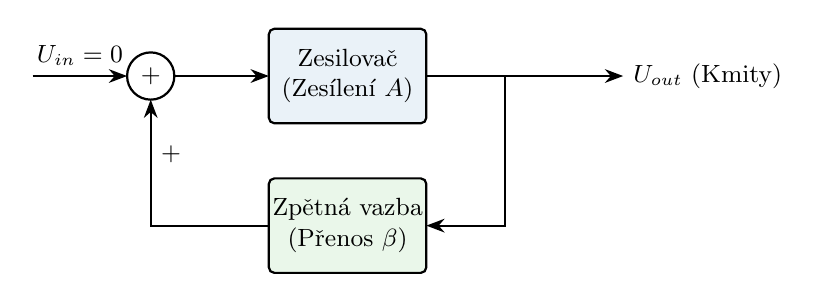
\begin{tikzpicture}[>=Stealth, font=\small, thick]
  % Součtový uzel
  \draw[fill=white] (0,0) circle (0.3) node {$+$};
  \draw[->] (-1.5,0) -- (-0.3,0) node[midway, above] {$U_{in} = 0$};

  % Zesilovač
  \draw[fill=lightblue, rounded corners=2pt] (1.5,-0.6) rectangle (3.5,0.6);
  \node[align=center] at (2.5,0) {Zesilovač\\(Zesílení $A$)};

  % Propojení uzlu a zesilovače
  \draw[->] (0.3,0) -- (1.5,0);

  % Výstup
  \draw[->] (3.5,0) -- (6,0) node[right] {$U_{out}$ (Kmity)};

  % Zpětná vazba
  \draw[fill=lightgreen, rounded corners=2pt] (1.5,-2.5) rectangle (3.5,-1.3);
  \node[align=center] at (2.5,-1.9) {Zpětná vazba\\(Přenos $\beta$)};

  \draw[->] (4.5,0) -- (4.5,-1.9) -- (3.5,-1.9);
  \draw[->] (1.5,-1.9) -- (0,-1.9) -- (0,-0.3);
  \node[right] at (0,-1) {$+$};
\end{tikzpicture}
\end{center}

\begin{durazbox}
\textbf{Barkhausenova podmínka nasazení kmitů:}
Aby oscilátor začal kmitat a udržel se, musí platit:
\begin{enumerate}
    \item \textbf{Amplitudová podmínka:} $A \cdot \beta \ge 1$ (Smyčkové zesílení musí být minimálně 1, ztráty se musí vyrovnat).
    \item \textbf{Fázová podmínka:} $\varphi = 0^\circ$ nebo $360^\circ$ (Signál se musí ze zpětné vazby vracet přesně ve fázi, aby se sčítal).
\end{enumerate}
\end{durazbox}

% ================================================================
\subsection*{2. Základní typy oscilátorů}

Oscilátory dělíme podle toho, jaké součástky určují jejich rezonanční frekvenci.

\begin{itemize}
    \item \textbf{RC oscilátory:} Určují frekvenci pomocí sítě rezistorů a kondenzátorů. Využívají se pro **nízké frekvence** (audio pásmo, Hz až desítky kHz). Příklad: \textit{Oscilátor s fázovým posuvem, Wienův článek}.
    \item \textbf{LC oscilátory:} Rezonančním obvodem je cívka a kondenzátor (paralelní LC obvod). Využívají se pro **vysoké frekvence** (rádio, MHz). Příklad: \textit{Colpittsův, Hartleyho oscilátor}.
    \item \textbf{Krystalové oscilátory (XTAL):} Využívají **piezoelektrický jev** výbrusu křemenného krystalu. Krystal funguje jako extrémně přesný LC obvod. Mají \textbf{obrovskou frekvenční stabilitu}. Tvoří hodiny (taktování) pro všechny procesory a hodinky (typicky $32{,}768\,\mathrm{kHz}$ pro reálný čas).
\end{itemize}

% ================================================================
\subsection*{3. Co je to Modulace a proč ji potřebujeme?}

\textbf{Modulace} je proces, při kterém se nízkofrekvenční informační signál (tzv. modulační signál - např. hlas, hudba, data) "vtiskne" do vysokofrekvenčního signálu (tzv. \textbf{nosná vlna} - carrier).

\textbf{Proč nemůžeme vysílat anténou rovnou lidský hlas (např. 1 kHz)?}
\begin{enumerate}
    \item \textbf{Délka antény:} Aby byla anténa účinná, musí být její délka ideálně $\lambda / 4$. Pro 1 kHz je vlnová délka $\lambda = 300\,000\,\mathrm{km/s} / 1\,000\,\mathrm{Hz} = 300\,\mathrm{km}$. Anténa by musela být dlouhá 75 kilometrů! Zvýšením frekvence nosné vlny na 100 MHz se anténa zkrátí na přijatelných 75 cm.
    \item \textbf{Překrývání stanic:} Všichni lidé mluví ve stejném frekvenčním pásmu. Bez modulace bychom v rádiu slyšeli všechny stanice najednou.
\end{enumerate}

% ================================================================
\subsection*{4. Analogové modulace (AM a FM)}

Při modulaci můžeme u nosné vlny ($u(t) = U_m \cdot \sin(\omega t + \varphi)$) měnit tři parametry: amplitudu ($U_m$), úhlovou frekvenci ($\omega$) nebo fázi ($\varphi$).

\begin{center}
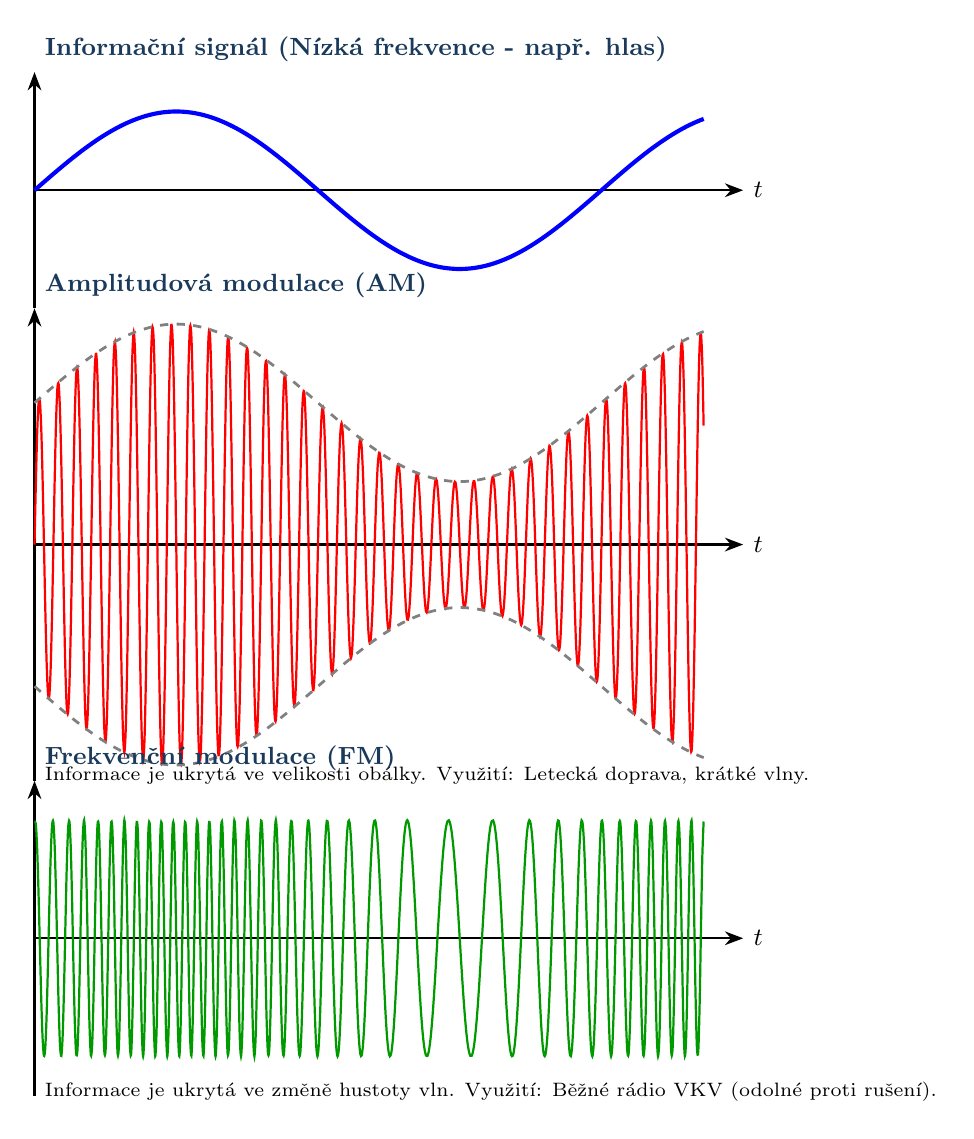
\begin{tikzpicture}[>=Stealth, font=\small, thick]
  % Vylepšené matematické funkce (Zvětšený modulační index pro jasnou FM změnu)
  \tikzset{declare function={
    mod_sig(\x) = sin(\x*50);
    am_sig(\x)  = (1.8 + mod_sig(\x)) * sin(\x*1500);
    fm_sig(\x)  = 1.5*sin(\x*1500 - 1000*cos(\x*50));
  }}

  % 1. Informační signál
  \draw[->] (0, 9) -- (9, 9) node[right] {$t$};
  \draw[->] (0, 7.5) -- (0, 10.5);
  \node[above right, accent] at (0, 10.5) {\textbf{Informační signál (Nízká frekvence - např. hlas)}};
  \draw[blue, line width=1.5pt, smooth, samples=150, domain=0:8.5] plot (\x, {9 + mod_sig(\x)});

  % 2. AM Modulace
  \draw[->] (0, 4.5) -- (9, 4.5) node[right] {$t$};
  \draw[->] (0, 1.5) -- (0, 7.5);
  \node[above right, accent] at (0, 7.5) {\textbf{Amplitudová modulace (AM)}};
  \draw[red, line width=0.8pt, smooth, samples=500, domain=0:8.5] plot (\x, {4.5 + am_sig(\x)});
  % Vykreslení obálky
  \draw[gray, dashed, line width=1pt, smooth, samples=150, domain=0:8.5] plot (\x, {4.5 + 1.8 + mod_sig(\x)});
  \draw[gray, dashed, line width=1pt, smooth, samples=150, domain=0:8.5] plot (\x, {4.5 - 1.8 - mod_sig(\x)});
  \node[below right, font=\scriptsize] at (0,1.8) {Informace je ukrytá ve velikosti obálky. Využití: Letecká doprava, krátké vlny.};

  % 3. FM Modulace
  \draw[->] (0, -0.5) -- (9, -0.5) node[right] {$t$};
  \draw[->] (0, -2.5) -- (0, 1.5);
  \node[above right, accent] at (0, 1.5) {\textbf{Frekvenční modulace (FM)}};
  \draw[green!60!black, line width=0.8pt, smooth, samples=500, domain=0:8.5] plot (\x, {-0.5 + fm_sig(\x)});
  \node[below right, font=\scriptsize] at (0,-2.2) {Informace je ukrytá ve změně hustoty vln. Využití: Běžné rádio VKV (odolné proti rušení).};

\end{tikzpicture}
\end{center}

% ================================================================
\subsection*{5. Demodulace (Detekce)}

Demodulátor přijímá vysokofrekvenční namodulovaný signál z antény a **získává z něj zpět původní užitečnou informaci** (nízkou frekvenci do reproduktoru).

\textbf{Obálkový detektor (Demodulátor AM):}\\
Je to ten nejjednodušší obvod používaný už v prvních rádiích (krystalkách). Skládá se z usměrňovací diody a kondenzátoru zapojeného paralelně s rezistorem.

\begin{enumerate}
    \item **Dioda** propustí jen kladnou polovinu vysokofrekvenčního AM signálu.
    \item **Kondenzátor $C$** se rychle nabije na špičkovou hodnotu vlny.
    \item V mezeře mezi vysokofrekvenčními kmity se kondenzátor pomalu vybíjí přes rezistor $R$. Pokud je časová konstanta správně zvolená, napětí na kondenzátoru dokonale opíše pomalou **obálku** původního signálu.
\end{enumerate}

\begin{center}
\begin{circuitikz}[font=\small, thick]
  % Vstupní AM signál
  \draw (0, 2) to[short, o-] (1, 2);
  \draw (0, 0) to[short, o-] (1, 0);
  \node[left] at (0, 1) {AM signál};
  \node[left] at (0, 2) {+};
  \node[left] at (0, 0) {--};

  % Transformátor / Anténní vstup
  \draw (1, 2) to[L, l=Cívka obvodu] (1, 0);

  % Dioda
  \draw (1, 2) to[D, l=Detekční dioda] (4, 2);

  % RC Filtr
  \draw (4, 2) to[C, l=$C$, *-*] (4, 0);
  \draw (6, 2) to[R, l=$R$, *-*] (6, 0);
  \draw (1, 0) -- (8, 0);
  \draw (4, 2) -- (8, 2);

  % Výstup
  \draw (8, 2) to[short, -o] (9, 2);
  \draw (8, 0) to[short, -o] (9, 0);
  \node[right, align=left] at (9, 1) {NF Signál\\(Obálka)};

  % Znázornění vyhlazení
  \draw[accent, dashed] (7.5, 2.5) sin (8, 2.8) cos (8.5, 2.5);
  \node[above] at (8, 2.8) {Užitečný zvuk};
\end{circuitikz}
\end{center}

\begin{durazbox}
\textbf{Digitální modulace (Moderní systémy - Wi-Fi, 5G, DVB-T):}
Dnes se analogové modulace (AM/FM) na ústupu. Informace z jedniček a nul se kóduje složitějšími metodami:
\begin{itemize}
    \item \textbf{ASK (Amplitude Shift Keying):} Přepínání amplitudy (např. 1 = velká amplituda, 0 = malá).
    \item \textbf{FSK (Frequency Shift Keying):} Přepínání dvou různých frekvencí (Bluetooth).
    \item \textbf{QAM (Kvadraturní amplitudová modulace):} Extrémně komplexní metoda měnící amplitudu i fázi současně, umožňuje přenášet mnoho bitů v jednom taktu.
\end{itemize}
\end{durazbox}

\end{vysvetlenibox}

\end{document}
